\documentclass[14pt, a4paper]{extarticle}

\usepackage[utf8]{inputenc}
\usepackage[T1]{fontenc}
\usepackage{amsmath}
\usepackage{amssymb}
\usepackage{graphicx}
\usepackage[left=2.00cm, right=2.00cm, top=2.00cm, bottom=2.00cm]{geometry}
\usepackage[russian]{babel}

\usepackage{setspace}
\usepackage{fancyhdr}

\graphicspath{{img/}}

\RequirePackage{caption}
\captionsetup[figure]{justification=centering,name=Рисунок,labelsep=endash}

\usepackage{indentfirst}

\usepackage{float}

\usepackage{titlesec}
\titleformat{\section}{\normalfont\bfseries}{\thesection~}{0em}{}

\begin{document}
	\onehalfspacing
	\begin{titlepage}
	\begin{center}
		\begin{small}
			\textbf{Министерство науки и высшего образования Российской Федерации}

			ФЕДЕРАЛЬНОЕ ГОСУДАРСТВЕННОЕ АВТОНОМНОЕ ОБРАЗОВАТЕЛЬНОЕ УЧРЕЖДЕНИЕ ВЫСШЕГО ОБРАЗОВАНИЯ
			
			\textbf{<<НАЦИОНАЛЬНЫЙ ИССЛЕДОВАТЕЛЬСКИЙ УНИВЕРСИТЕТ ИТМО>>}
		\end{small}
		
		\vspace{8em}
		
		Отчет по лабораторной работе №4
		
		РОБАСТНОЕ УПРАВЛЕНИЕ ЛИНЕЙНЫМ МНОГОМЕРНЫМ ОБЪЕКТОМ ПО СОСТОЯНИЮ
		
		По дисциплине <<Адаптивное и робастное управление>>
	\end{center}
	
	\vspace{8em}
	
	\begin{flushright}
		Выполнил:\\
		студент группы R42331c\\
		Манахов~С.П.
		
		\vspace{1em}
		
		Преподаватель:\\
		Парамонов~А.В.
	\end{flushright}

	\vfill
	
	\begin{center}
		\small
		Санкт-Петербург\\
		2022 г.\\
	\end{center}
\end{titlepage}
	\setcounter{page}{2}
	
	\section*{Задание}
	
	Дан возмущенный объект, модель которого описывается уравнениями вида:
	$$\begin{matrix}
		\dot{x} = Ax + bu + \delta, x(0),\\
		y = Cx,
	\end{matrix}$$
	где $\delta$ -- вектор возмущающих воздействий, удовлетворяющий неравенству $\left|\left|\delta(t)\right|\right|\le \bar{\delta}$. В модели $x\in R^n$ -- вектор состояния, $y$ -- регулируемая переменная, матрицы $A$, $b$ и $C$ идентичны соответствующим матрицам объекта из работы~№3.
	
	Цель управления заключается в обеспечении целевого неравенства:
	$$\left|\left|x_M(t)-x(t)\right|\right|\le\Delta, \forall t \ge T,$$
	где $\Delta, T$ -- точность работы системы управления и время ее настройки соответственно, $x_M(t)\in R^n$ -- эталонный сигнал, генерируемый моделью из работы~№3.

	\begin{enumerate}
		\item На основе результатов, полученных при выполнении работы~№3, модифицировать алгоритм адаптации и сформировать закон нелинейного робастного управления и закон адаптивного и робастного управления. Построить в пакете \textit{Simulink} модели соответствующих замкнутых систем управления, приняв в качестве возмущения следующую вектор-функцию:
		$$\delta(t)=\left[\begin{matrix}
			0,6sin10t+0,1sin50t, & 0,5cos12t+0,2sin30t
		\end{matrix}\right]^T$$
		\item Провести эксперименты с системой робастного управления, замкнутой алгоритмом:
		$$\hat{\theta}=\gamma xb^TPe$$
		для трех различных коэффициентов $\gamma$ при отсутствии и наличии возмущения $\delta(t)$.
		
		По результатам каждого эксперимента построить траектории $x(t)$ и $x_M(t)$ на одном графике, $e(t)$ -- на другом;
		\item Провести эксперименты с системой робастного управления, замкнутой алгоритмом:
		$$\dot{\hat{\theta}}=-\sigma\hat{\theta}+\gamma xb^TPe$$
		для выбранного параметра $\sigma$ и двух различных коэффициентов $\gamma$, принятых в п.п.~2, при отсутствии и наличии возмущения $\delta(t)$. Далее уменьшить параметр $\sigma$ и повторить предыдущий эксперимент (при отсутствии и наличии возмущения $\delta(t)$) для одного из выбранных коэффициентов $\gamma$.
		
		По результатам каждого эксперимента построить траектории $x(t)$ и $x_M(t)$ на одном графике, $e(t)$ -- на втором и $\tilde{\theta}(t)$ -- на третьем;
		\item Сделать выводы по каждому пункту работы.
 	\end{enumerate}
	\begin{table}[H]
		\centering
		\begin{tabular}{|l|l|p{0.1\textwidth}|p{0.13\textwidth}|p{0.2\textwidth}|p{0.15\textwidth}|}
			\hline
			Вариант & Матрица $A$ & Коэф передачи $b_0$ & Время переходного процесса, $t_n$ & Максимального перерегулирование $\bar{\sigma}$, \% & Сигнал задания $g(t)$\\\hline
			18 & 
			$\left[
			\begin{matrix}
				0 & 1 \\
				-10 & 6 
			\end{matrix}
			\right]$
			& 9 & 0,15 & 15 & $0,8sin2t+cos0,8t+2$ \\\hline
		\end{tabular}
	\end{table}
	
	\newpage
	
	\section*{Описание работы}
	
	\begin{enumerate}
		\item Построенные в пакете \textit{Simulink} модели замкнутых систем управления с законом нелинейного робастного управления и законом адаптивного и робастного управления соответственно представлены на рисунках \ref{fig:2-system} и \ref{fig:3-system}, а также на рисунке \ref{fig:2-properties}.
		
		\begin{figure}[H]
			\centering
			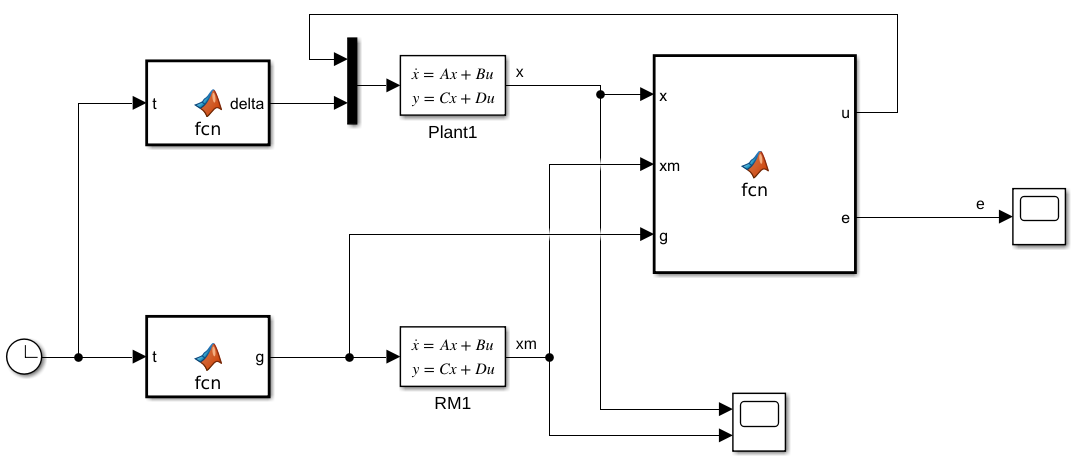
\includegraphics[width=0.59\textwidth]{2-system}
			\caption{Система с нелиненым законом робастного управления}
			\label{fig:2-system}
		\end{figure}
		
		\begin{figure}[H]
			\centering
			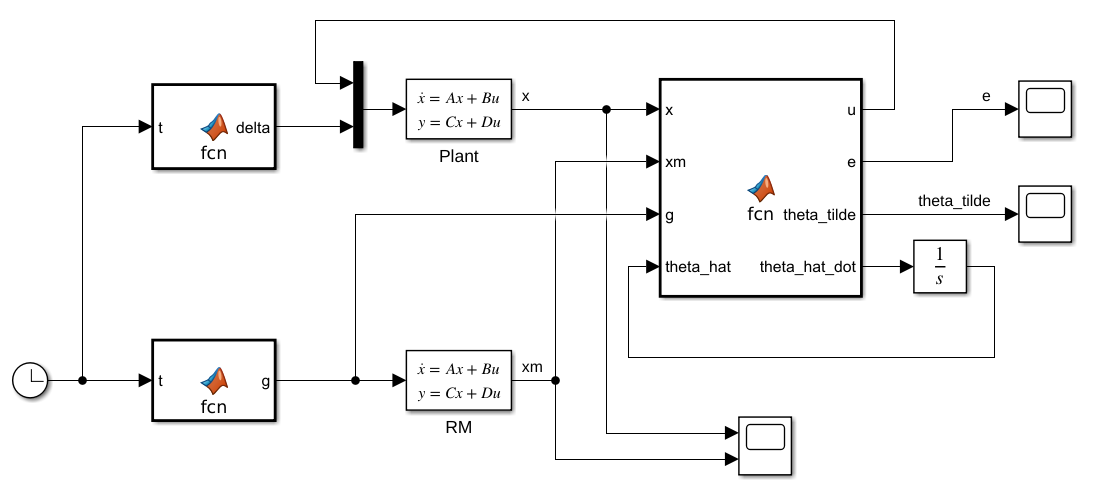
\includegraphics[width=0.59\textwidth]{3-system}
			\caption{Система с законом адаптивного и робастного управления}
			\label{fig:3-system}
		\end{figure}
	
		\begin{figure}[H]
			\centering
			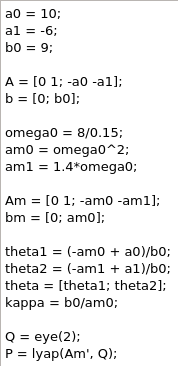
\includegraphics{2-properties}
			\caption{Параметры системы}
			\label{fig:2-properties}
		\end{figure}
		
		\item Примем $\gamma=100$ и промоделируем систему с законом нелинейного робастного управления при отсутствии возмущения $\delta(t)$. Полученные графики представлены на рисунках \ref{fig:2-1-x}, \ref{fig:2-1-e}.
		
		\begin{figure}[H]
			\centering
			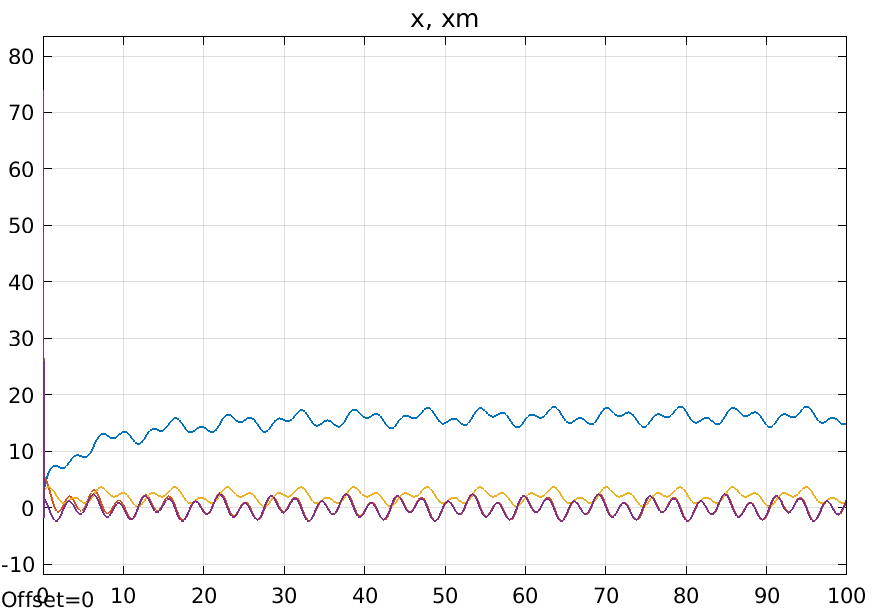
\includegraphics[width=0.59\textwidth]{2-1-x}
			\caption{Векторы $x$ и $x_M$ при $\gamma=100$ и отсутствии $\delta(t)$}
			\label{fig:2-1-x}
		\end{figure}
		
		\begin{figure}[H]
			\centering
			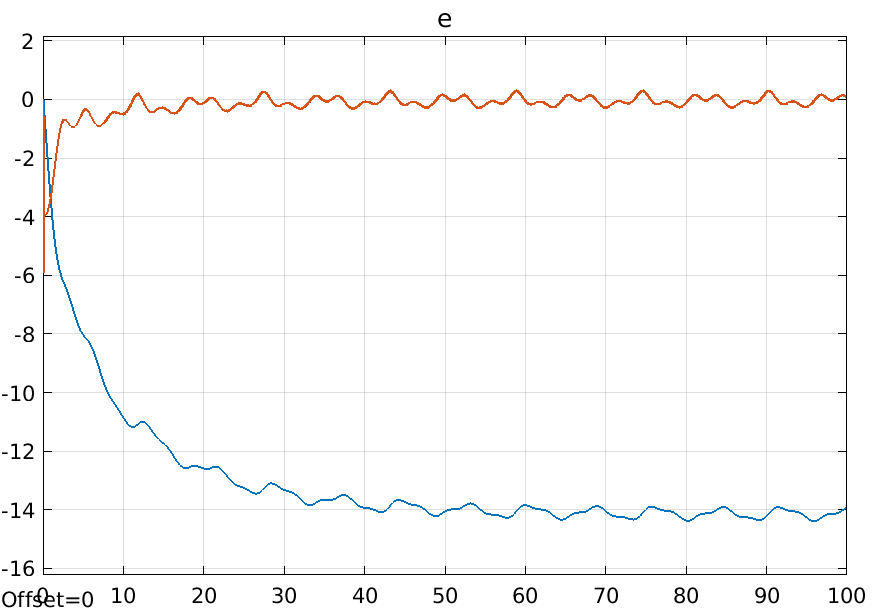
\includegraphics[width=0.59\textwidth]{2-1-e}
			\caption{Вектор $e$ при $\gamma=100$ и отсутствии $\delta(t)$}
			\label{fig:2-1-e}
		\end{figure}
		
		Теперь промоделируем при наличии возмущения $\delta(t)$. Полученные графики представлены на рисунках \ref{fig:2-2-x}, \ref{fig:2-2-e}.
		
		\begin{figure}[H]
			\centering
			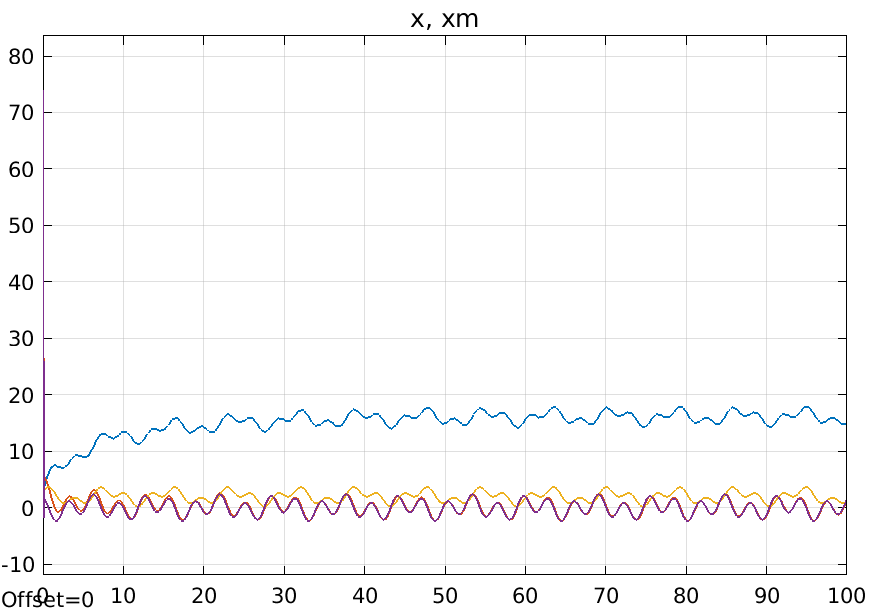
\includegraphics[width=0.59\textwidth]{2-2-x}
			\caption{Векторы $x$ и $x_M$ при $\gamma=100$ и наличии $\delta(t)$}
			\label{fig:2-2-x}
		\end{figure}
		
		\begin{figure}[H]
			\centering
			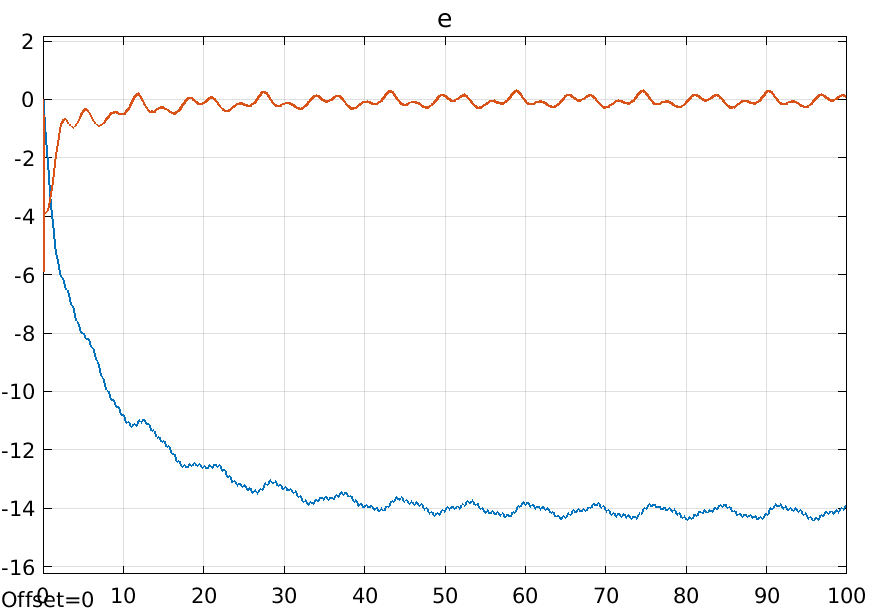
\includegraphics[width=0.59\textwidth]{2-2-e}
			\caption{Вектор $e$ при $\gamma=100$ и наличии $\delta(t)$}
			\label{fig:2-2-e}
		\end{figure}
		
		Примем $\gamma=200$ и промоделируем систему при отсутствии возмущения $\delta(t)$. Полученные графики представлены на рисунках \ref{fig:2-3-x}, \ref{fig:2-3-e}.
		
		\begin{figure}[H]
			\centering
			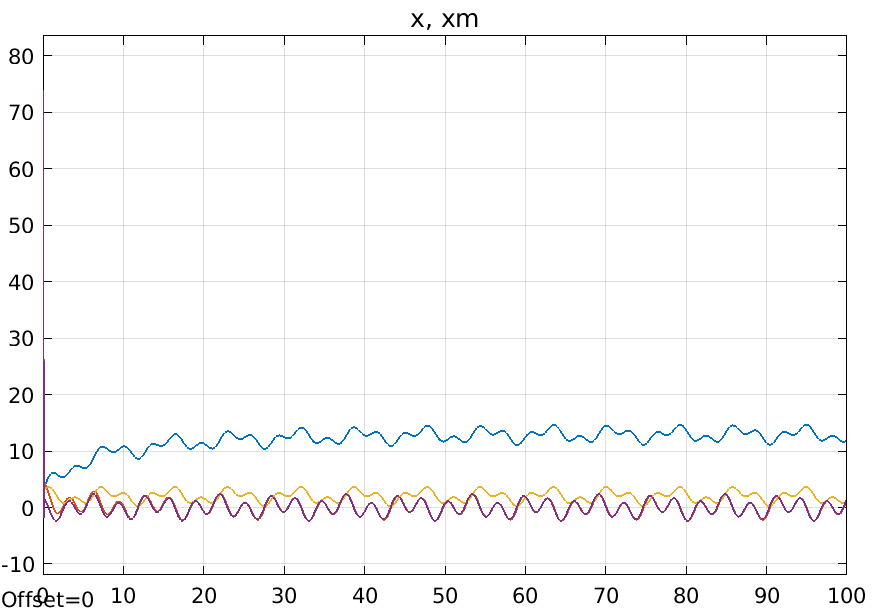
\includegraphics[width=0.59\textwidth]{2-3-x}
			\caption{Векторы $x$ и $x_M$ при $\gamma=200$ и отсутствии $\delta(t)$}
			\label{fig:2-3-x}
		\end{figure}
		
		\begin{figure}[H]
			\centering
			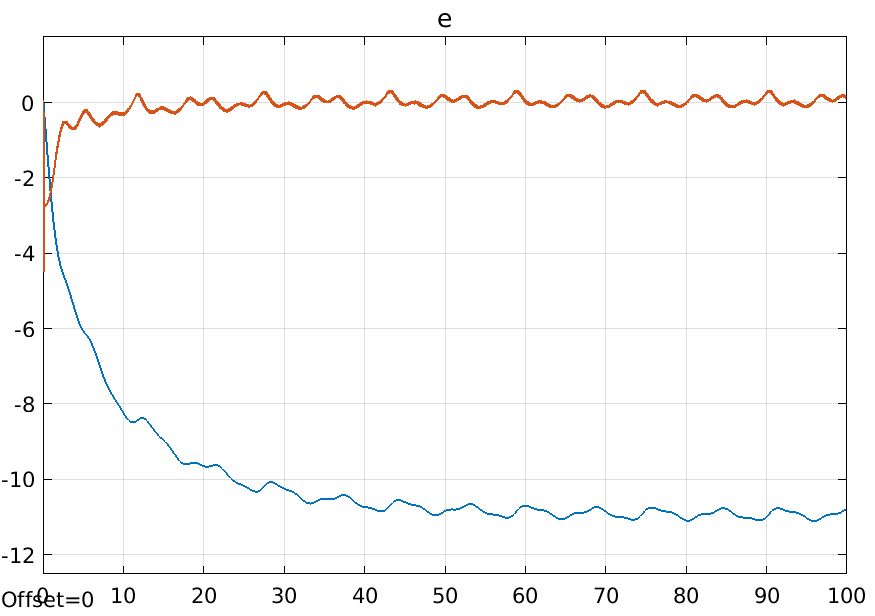
\includegraphics[width=0.59\textwidth]{2-3-e}
			\caption{Вектор $e$ при $\gamma=200$ и отсутствии $\delta(t)$}
			\label{fig:2-3-e}
		\end{figure}
		
		Теперь промоделируем при наличии возмущения $\delta(t)$. Полученные графики представлены на рисунках \ref{fig:2-4-x}, \ref{fig:2-4-e}.
		
		\begin{figure}[H]
			\centering
			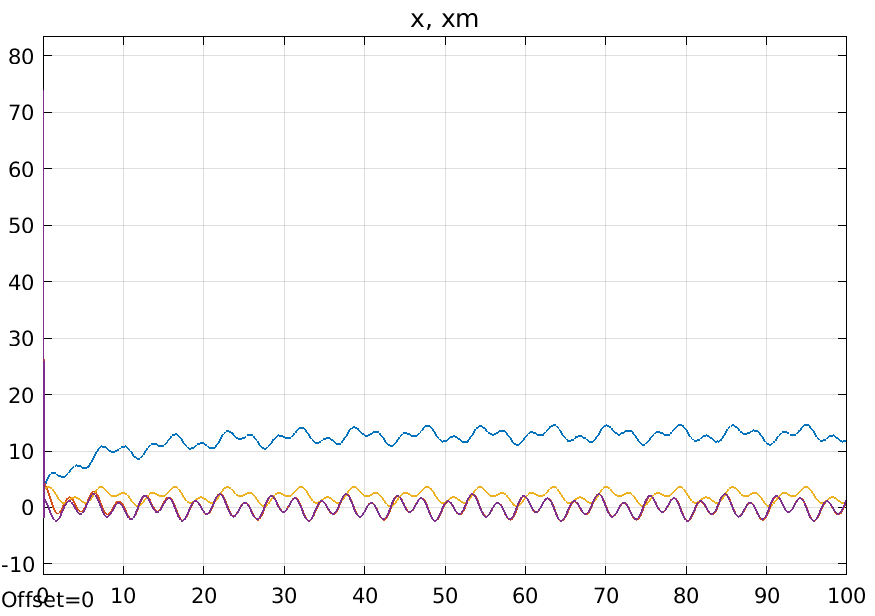
\includegraphics[width=0.59\textwidth]{2-4-x}
			\caption{Векторы $x$ и $x_M$ при $\gamma=200$ и наличии $\delta(t)$}
			\label{fig:2-4-x}
		\end{figure}
		
		\begin{figure}[H]
			\centering
			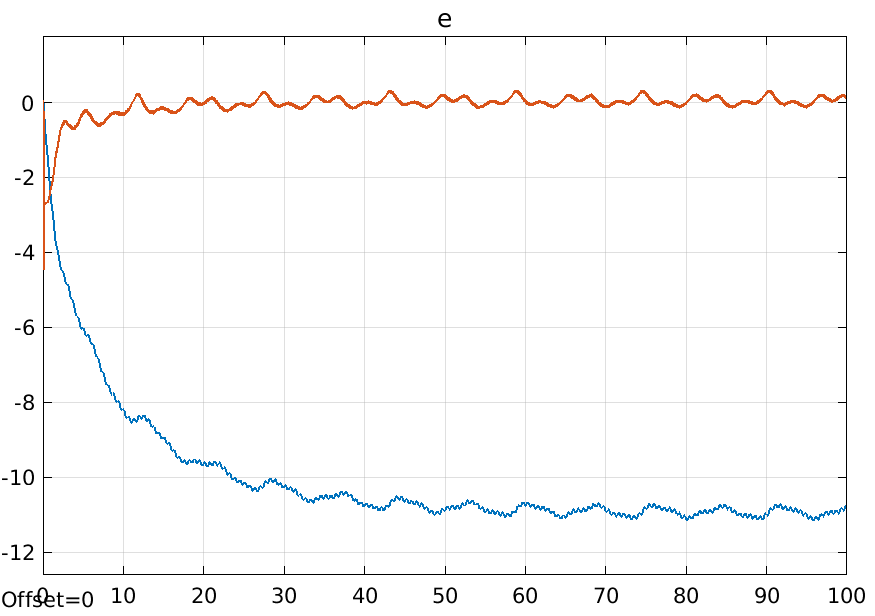
\includegraphics[width=0.59\textwidth]{2-4-e}
			\caption{Вектор $e$ при $\gamma=200$ и наличии $\delta(t)$}
			\label{fig:2-4-e}
		\end{figure}
		
		Примем $\gamma=1000$ и промоделируем систему при отсутствии возмущения $\delta(t)$. Полученные графики представлены на рисунках \ref{fig:2-5-x}, \ref{fig:2-5-e}.
		
		\begin{figure}[H]
			\centering
			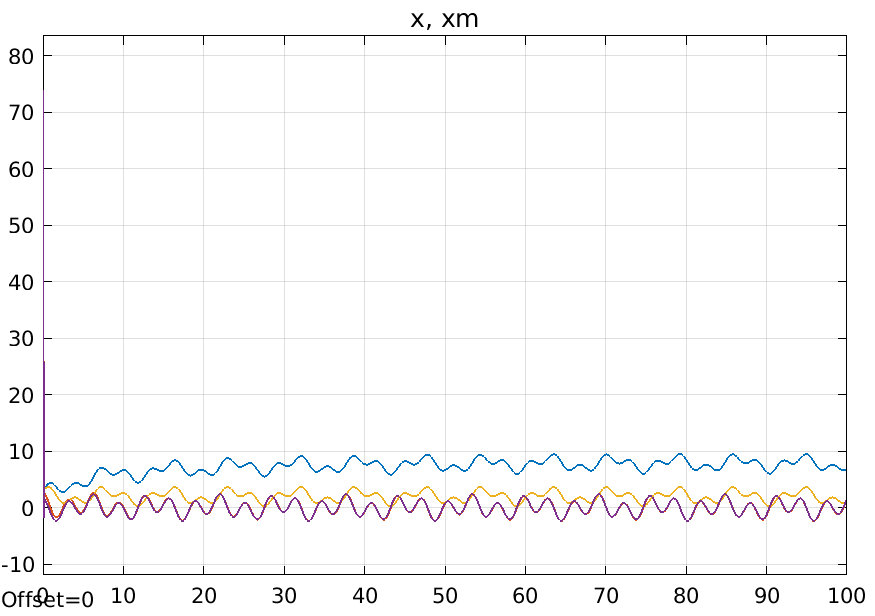
\includegraphics[width=0.59\textwidth]{2-5-x}
			\caption{Векторы $x$ и $x_M$ при $\gamma=1000$ и отсутствии $\delta(t)$}
			\label{fig:2-5-x}
		\end{figure}
		
		\begin{figure}[H]
			\centering
			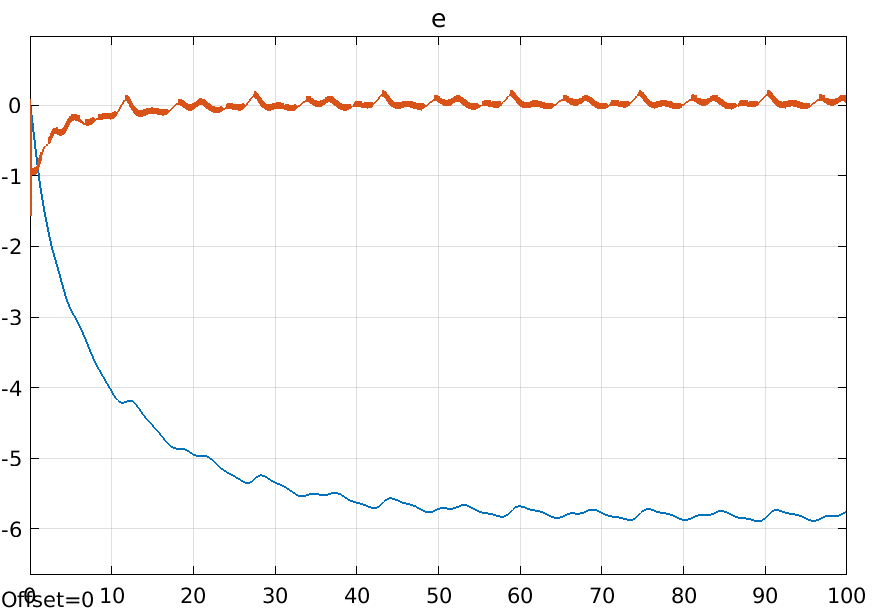
\includegraphics[width=0.59\textwidth]{2-5-e}
			\caption{Вектор $e$ при $\gamma=1000$ и отсутствии $\delta(t)$}
			\label{fig:2-5-e}
		\end{figure}
		
		Теперь промоделируем при наличии возмущения $\delta(t)$. Полученные графики представлены на рисунках \ref{fig:2-6-x}, \ref{fig:2-6-e}.
		
		\begin{figure}[H]
			\centering
			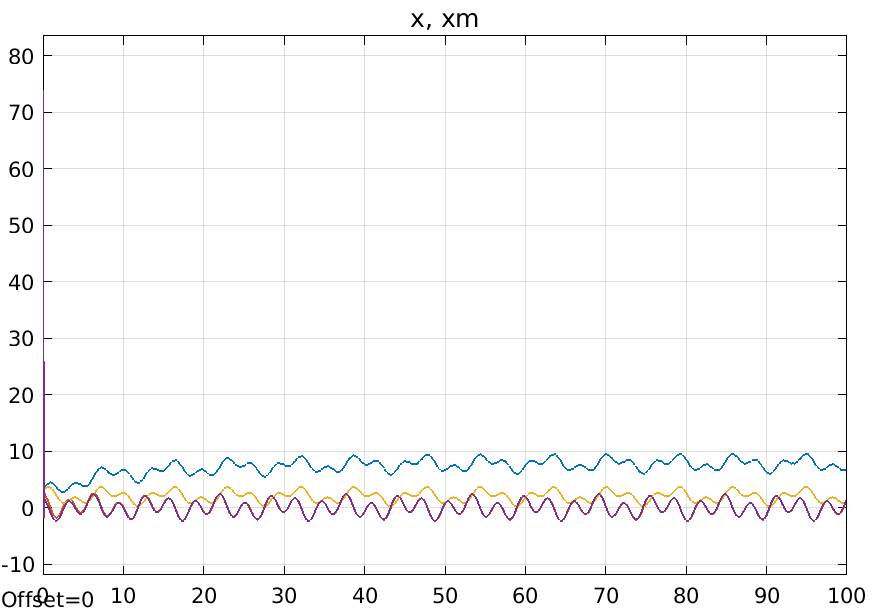
\includegraphics[width=0.59\textwidth]{2-6-x}
			\caption{Векторы $x$ и $x_M$ при $\gamma=1000$ и наличии $\delta(t)$}
			\label{fig:2-6-x}
		\end{figure}
		
		\begin{figure}[H]
			\centering
			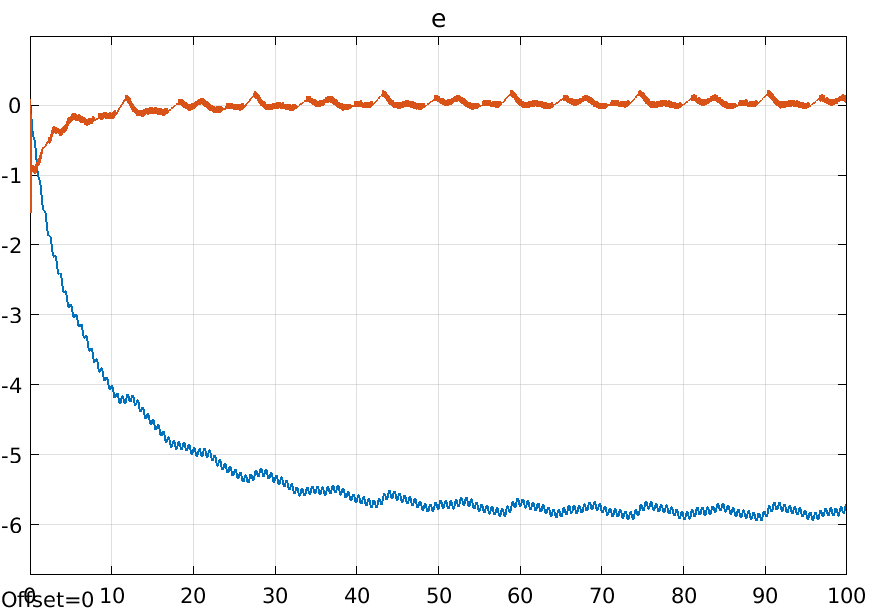
\includegraphics[width=0.59\textwidth]{2-6-e}
			\caption{Вектор $e$ при $\gamma=1000$ и наличии $\delta(t)$}
			\label{fig:2-6-e}
		\end{figure}
		
		\item Примем $\sigma=0,1$ и промоделируем систему с законом адаптивного и робастного управления при $\gamma=100$ и отсутствии возмущения $\delta(t)$. Полученные графики представлены на рисунках \ref{fig:3-1-x}-\ref{fig:3-1-theta}.
		
		\begin{figure}[H]
			\centering
			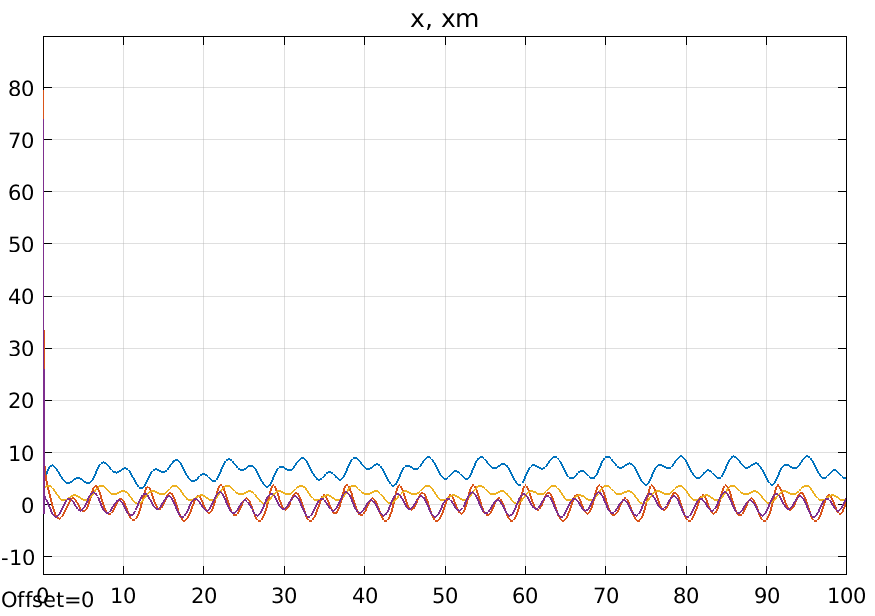
\includegraphics[width=0.59\textwidth]{3-1-x}
			\caption{Векторы $x$ и $x_M$ при $\gamma=100$ и отсутствии $\delta(t)$}
			\label{fig:3-1-x}
		\end{figure}
		
		\begin{figure}[H]
			\centering
			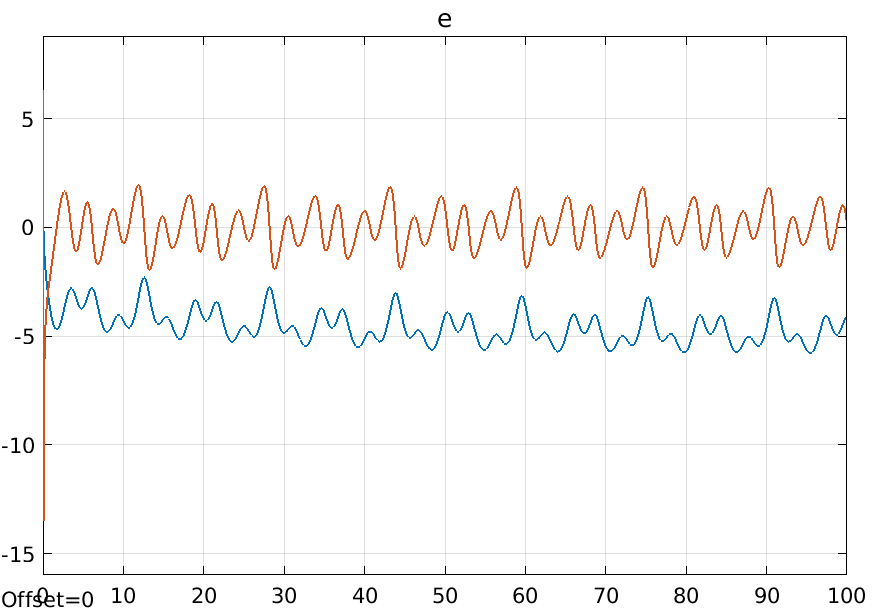
\includegraphics[width=0.59\textwidth]{3-1-e}
			\caption{Вектор $e$ при $\gamma=100$ и отсутствии $\delta(t)$}
			\label{fig:3-1-e}
		\end{figure}
		
		\begin{figure}[H]
			\centering
			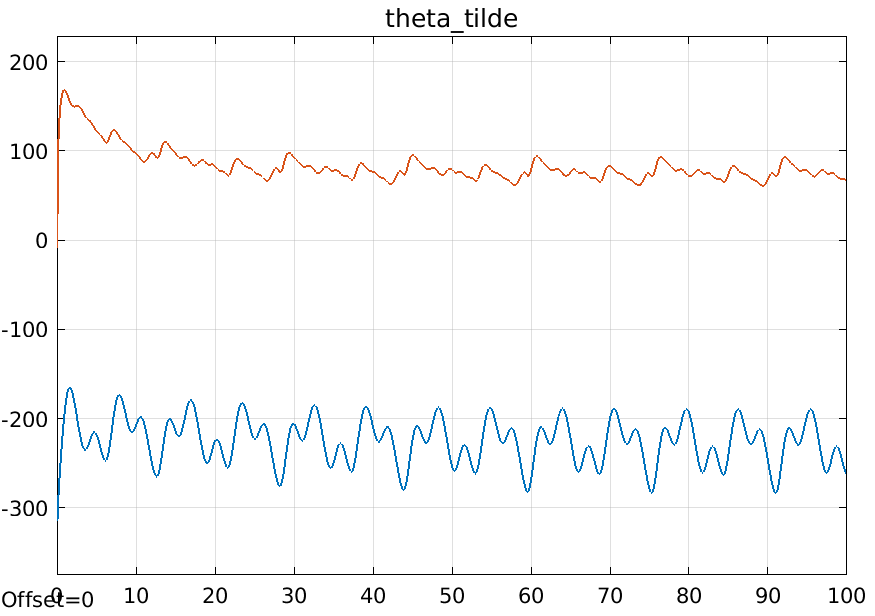
\includegraphics[width=0.59\textwidth]{3-1-theta}
			\caption{Вектор $\tilde{\theta}$ при $\gamma=100$ и отсутствии $\delta(t)$}
			\label{fig:3-1-theta}
		\end{figure}
		
		Теперь промоделируем при наличии возмущения $\delta(t)$. Полученные графики представлены на рисунках \ref{fig:3-2-x}-\ref{fig:3-2-theta}.
		
		\begin{figure}[H]
			\centering
			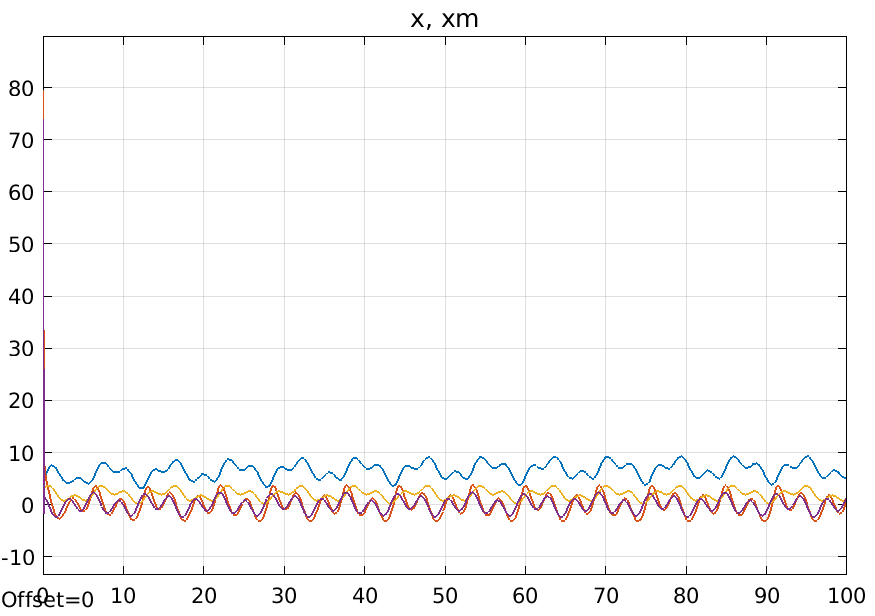
\includegraphics[width=0.59\textwidth]{3-2-x}
			\caption{Векторы $x$ и $x_M$ при $\gamma=100$ и наличии $\delta(t)$}
			\label{fig:3-2-x}
		\end{figure}
		
		\begin{figure}[H]
			\centering
			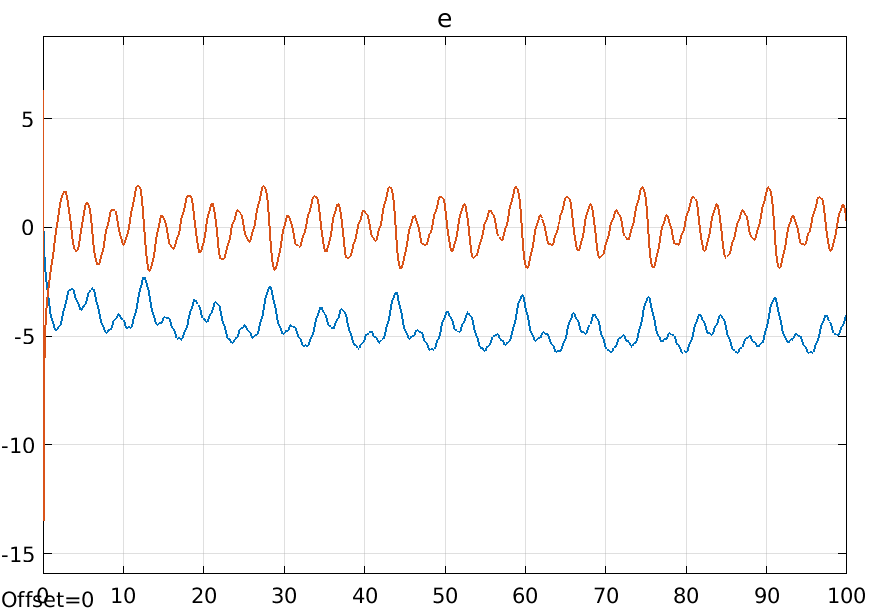
\includegraphics[width=0.59\textwidth]{3-2-e}
			\caption{Вектор $e$ при $\gamma=100$ и наличии $\delta(t)$}
			\label{fig:3-2-e}
		\end{figure}
		
		\begin{figure}[H]
			\centering
			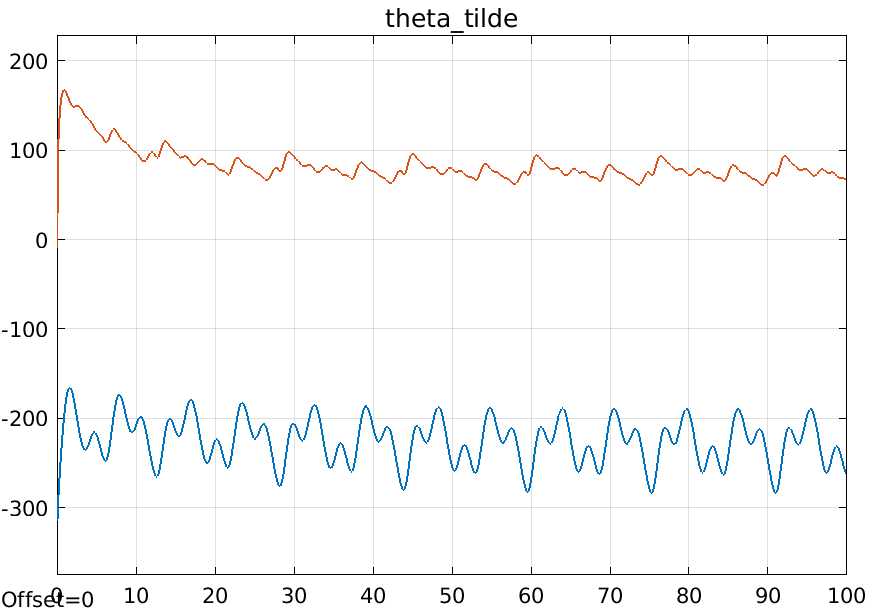
\includegraphics[width=0.59\textwidth]{3-2-theta}
			\caption{Вектор $\tilde{\theta}$ при $\gamma=100$ и наличии $\delta(t)$}
			\label{fig:3-2-theta}
		\end{figure}
		
		Не изменяя значение $\sigma$, примем $\gamma=1000$ и промоделируем систему при отсутствии возмущения $\delta(t)$. Полученные графики представлены на рисунках \ref{fig:3-3-x}-\ref{fig:3-3-theta}.
		
		\begin{figure}[H]
			\centering
			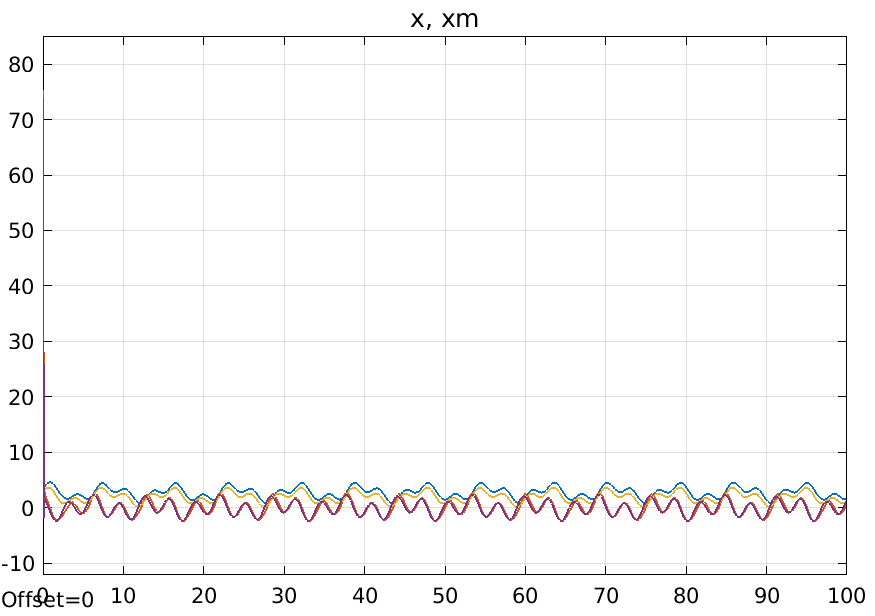
\includegraphics[width=0.59\textwidth]{3-3-x}
			\caption{Векторы $x$ и $x_M$ при $\gamma=1000$ и отсутствии $\delta(t)$}
			\label{fig:3-3-x}
		\end{figure}
		
		\begin{figure}[H]
			\centering
			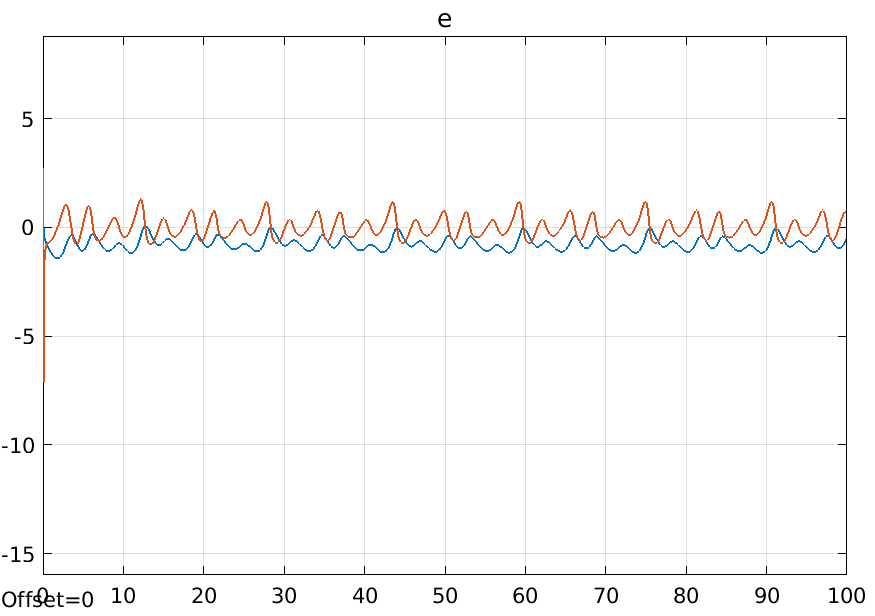
\includegraphics[width=0.59\textwidth]{3-3-e}
			\caption{Вектор $e$ при $\gamma=1000$ и отсутствии $\delta(t)$}
			\label{fig:3-3-e}
		\end{figure}
		
		\begin{figure}[H]
			\centering
			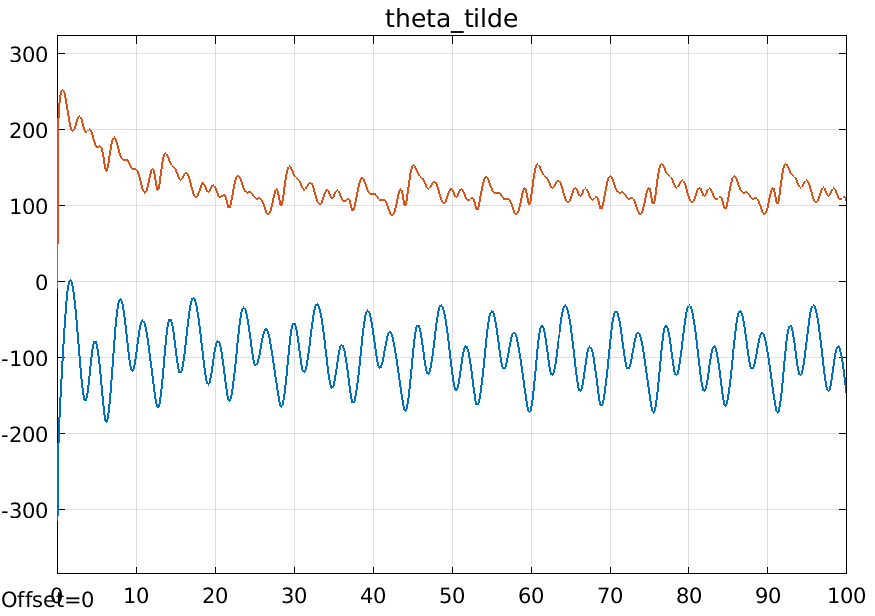
\includegraphics[width=0.59\textwidth]{3-3-theta}
			\caption{Вектор $\tilde{\theta}$ при $\gamma=1000$ и отсутствии $\delta(t)$}
			\label{fig:3-3-theta}
		\end{figure}
		
		Теперь промоделируем при наличии возмущения $\delta(t)$. Полученные графики представлены на рисунках \ref{fig:3-4-x}-\ref{fig:3-4-theta}.
		
		\begin{figure}[H]
			\centering
			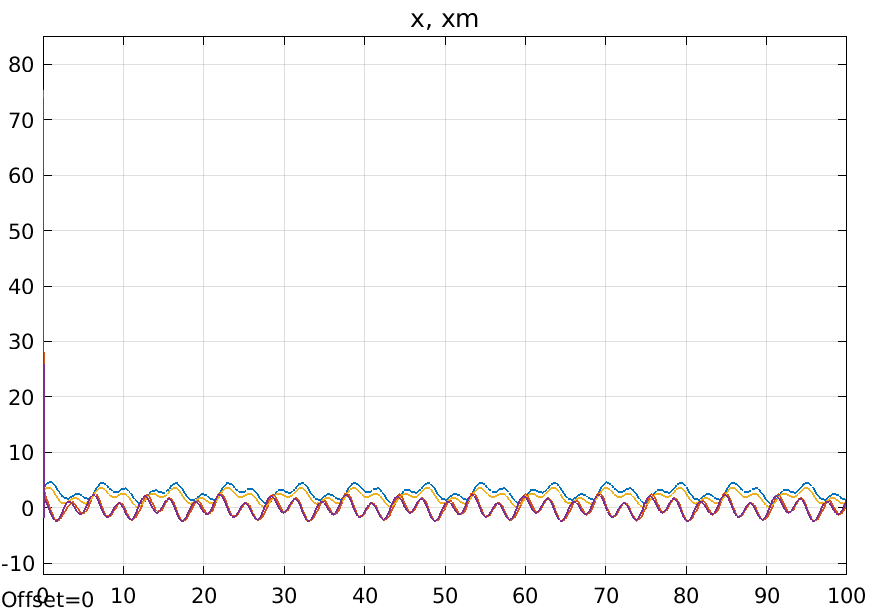
\includegraphics[width=0.59\textwidth]{3-4-x}
			\caption{Векторы $x$ и $x_M$ при $\gamma=1000$ и наличии $\delta(t)$}
			\label{fig:3-4-x}
		\end{figure}
		
		\begin{figure}[H]
			\centering
			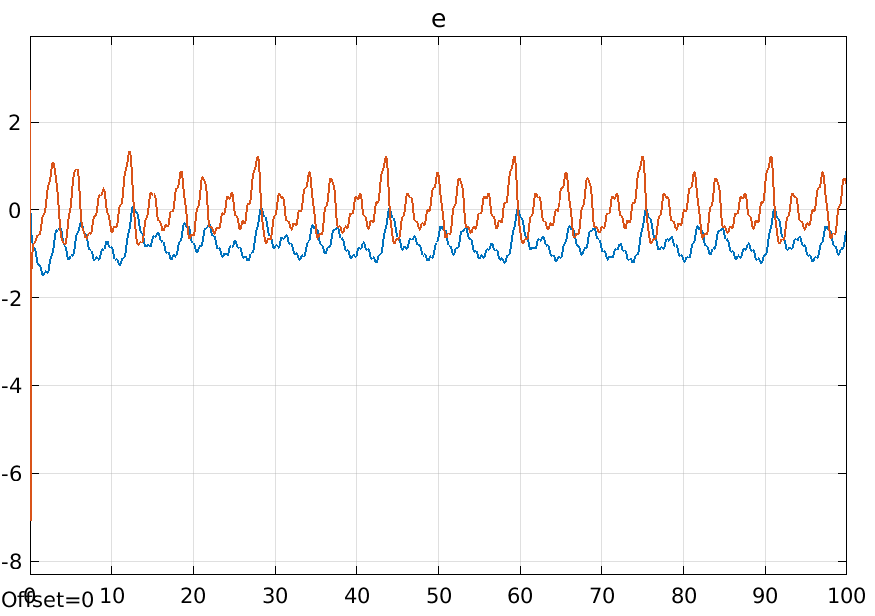
\includegraphics[width=0.59\textwidth]{3-4-e}
			\caption{Вектор $e$ при $\gamma=1000$ и наличии $\delta(t)$}
			\label{fig:3-4-e}
		\end{figure}
		
		\begin{figure}[H]
			\centering
			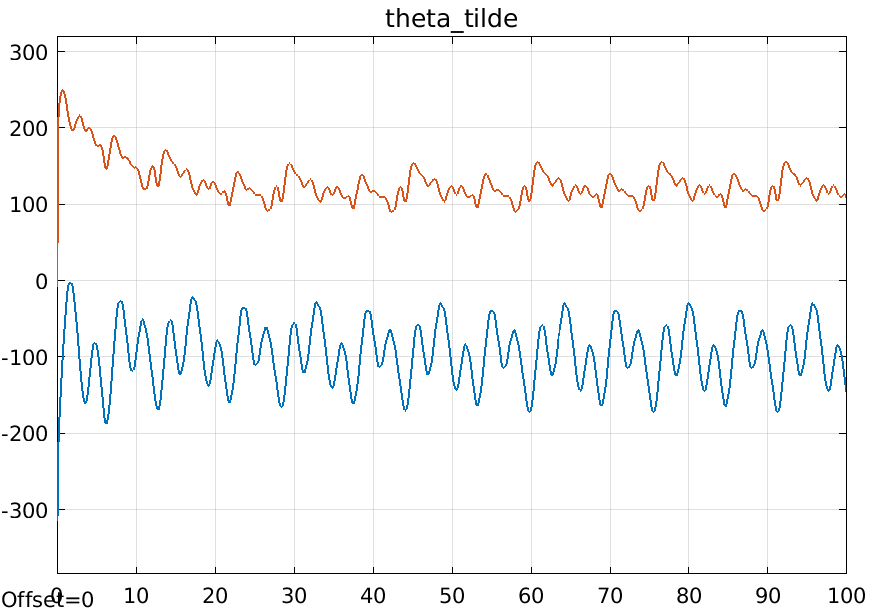
\includegraphics[width=0.59\textwidth]{3-4-theta}
			\caption{Вектор $\tilde{\theta}$ при $\gamma=1000$ и наличии $\delta(t)$}
			\label{fig:3-4-theta}
		\end{figure}
		
		Теперь уменьшим параметр $\sigma=0,01$ и промоделируем систему при $\gamma=100$ и отсутствии возмущения $\delta(t)$. Полученные графики представлены на рисунках \ref{fig:3-5-x}-\ref{fig:3-5-theta}.
		
		\begin{figure}[H]
			\centering
			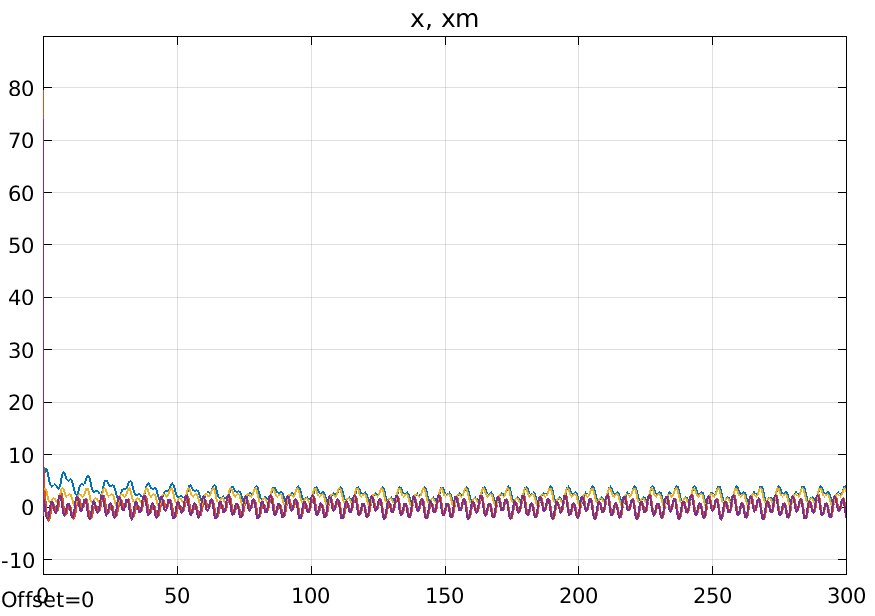
\includegraphics[width=0.59\textwidth]{3-5-x}
			\caption{Векторы $x$ и $x_M$ при $\sigma=0,01$ и отсутствии $\delta(t)$}
			\label{fig:3-5-x}
		\end{figure}
		
		\begin{figure}[H]
			\centering
			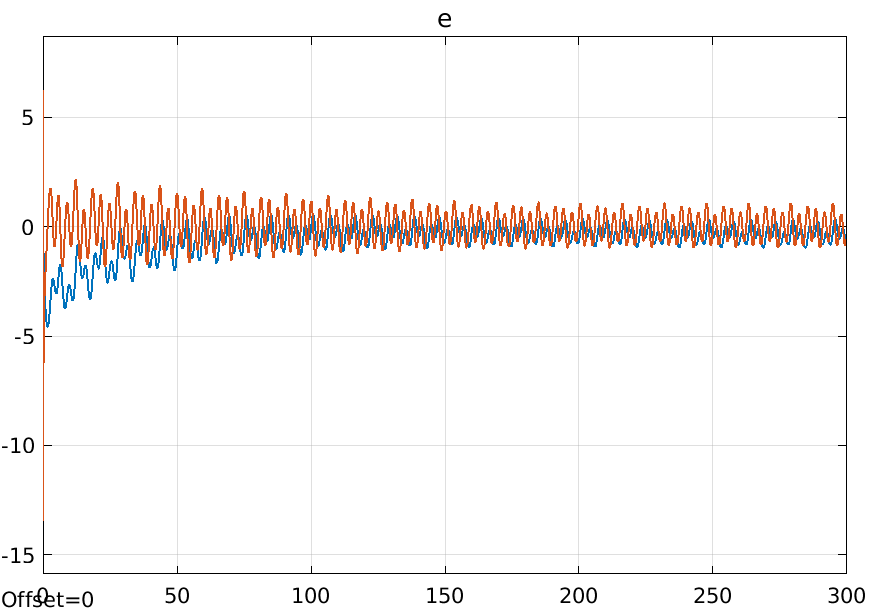
\includegraphics[width=0.59\textwidth]{3-5-e}
			\caption{Вектор $e$ при $\sigma=0,01$ и отсутствии $\delta(t)$}
			\label{fig:3-5-e}
		\end{figure}
		
		\begin{figure}[H]
			\centering
			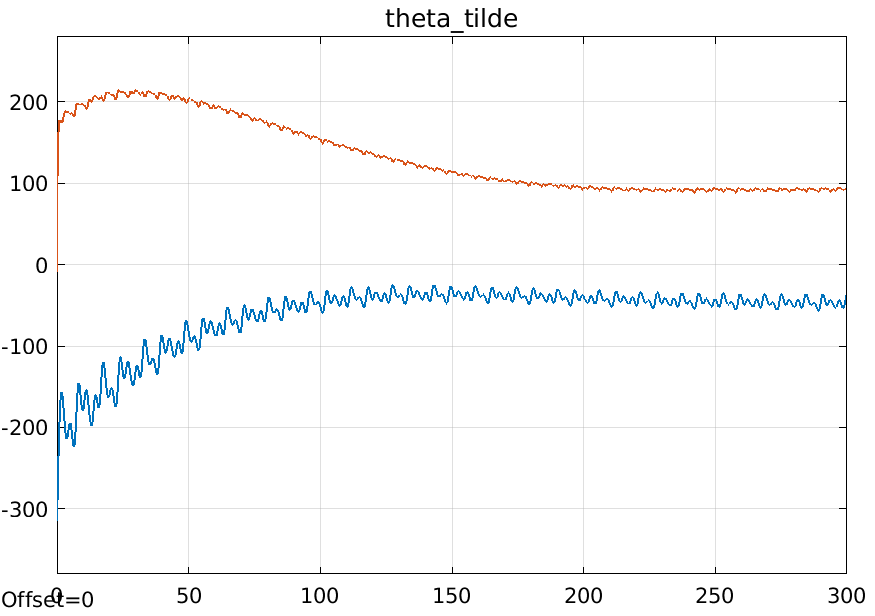
\includegraphics[width=0.59\textwidth]{3-5-theta}
			\caption{Вектор $\tilde{\theta}$ при $\sigma=0,01$ и отсутствии $\delta(t)$}
			\label{fig:3-5-theta}
		\end{figure}
		
		Теперь промоделируем при наличии возмущения $\delta(t)$. Полученные графики представлены на рисунках \ref{fig:3-6-x}-\ref{fig:3-6-theta}.
		
		\begin{figure}[H]
			\centering
			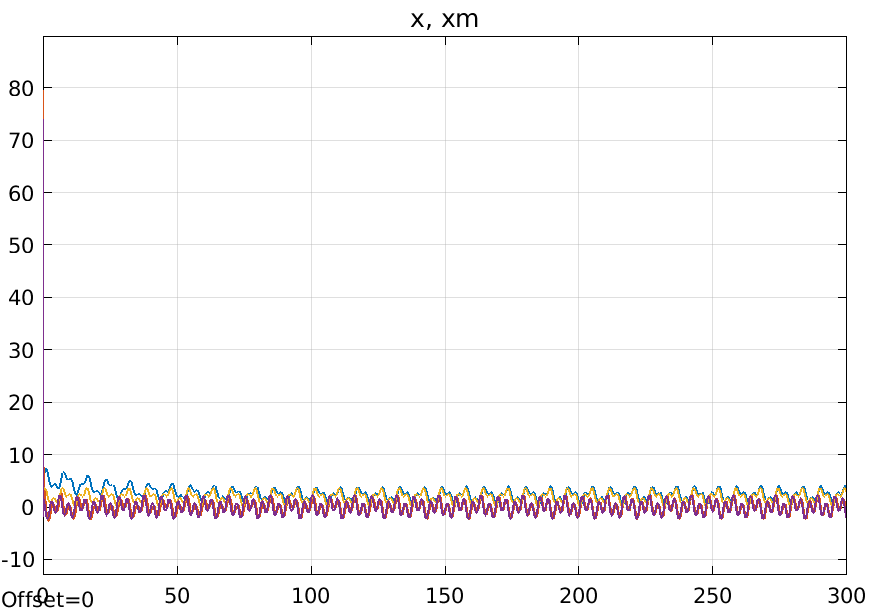
\includegraphics[width=0.59\textwidth]{3-6-x}
			\caption{Векторы $x$ и $x_M$ при $\sigma=0,01$ и наличии $\delta(t)$}
			\label{fig:3-6-x}
		\end{figure}
		
		\begin{figure}[H]
			\centering
			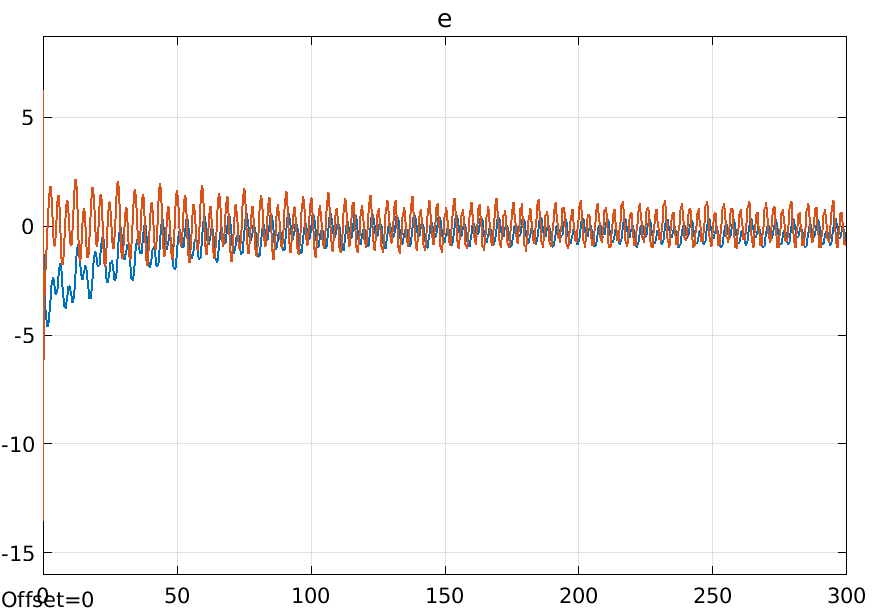
\includegraphics[width=0.59\textwidth]{3-6-e}
			\caption{Вектор $e$ при $\sigma=0,01$ и наличии $\delta(t)$}
			\label{fig:3-6-e}
		\end{figure}
		
		\begin{figure}[H]
			\centering
			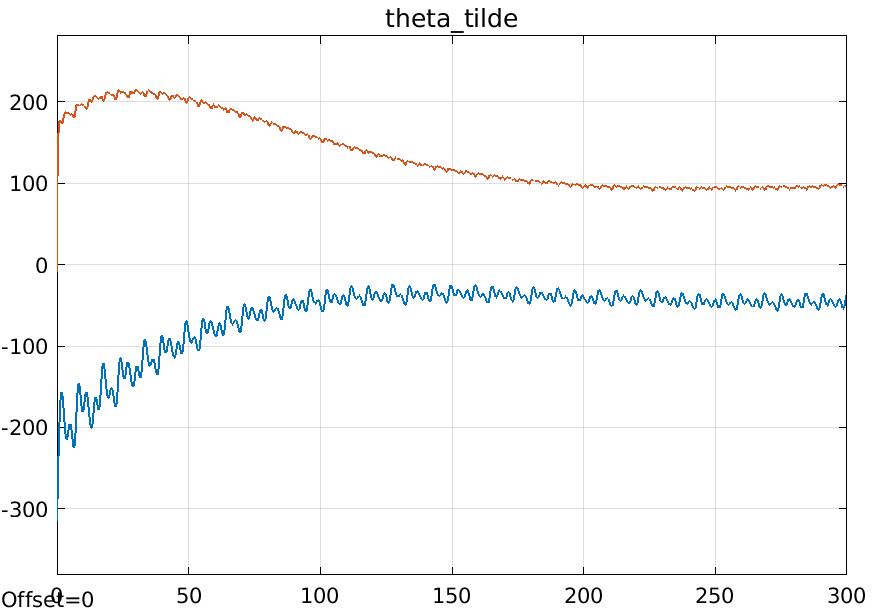
\includegraphics[width=0.59\textwidth]{3-6-theta}
			\caption{Вектор $\tilde{\theta}$ при $\sigma=0,01$ и наличии $\delta(t)$}
			\label{fig:3-6-theta}
		\end{figure}
		
	\end{enumerate}

	\newpage
	
	\section*{Вывод}
	
	Во время выполнения работы была доказана ограниченность всех сигналов.
	
	Также было показано, что при увеличении коэффициента $\gamma$ уменьшается радиус окрестности вектора ошибки $e$.
	
	А при снижении параметра $\sigma$ можно уменьшить радиус окрестности векторов ошибки $e$ и $\tilde{\theta}$.
	
	

\end{document}